    \documentclass[12pt,a4paper]{article}
\usepackage[margin=1in]{geometry}
\usepackage{booktabs}
\usepackage{setspace}
\usepackage{hyperref}
\usepackage{array}
\usepackage{longtable}
\usepackage{graphicx}
\usepackage{url} 


\onehalfspacing
\setcounter{secnumdepth}{4}

%=== COVER PAGE ===
\begin{document}
\begin{titlepage}
    \centering
    {\Large\bfseries CM10025 Programming 2: Personal Informatics System Report\par}
    \vspace{1cm}
    Group Name: Agile Analysts \\
    Group Number: 18 \\
    Date: March 24, 2025

    \vspace{2cm}
    \begin{tabular}{llll}
        \toprule
        Group Member & Username & Degree & Course \\
        \midrule
        David Cai & yc2800 & MComp Computer Science and Mathematics & Year 1 \\
        Mandeep Thakur & mt2434 &  MComp Computer Science and Mathematics & Year 1\\
        Jack Bancroft & jgb64 & BSc Computer Science & Year 1\\
        James Beagrie & jb4106 & BSc Computer Science and Mathematics & Year 1\\
        Satima Dosso & sd2745 & BSc Computer Science and Mathematics & Year 1 \\
        Bhuvan Kumar & bk597 & BSc Computer Science & Year 1\\
    \end{tabular}
    \thispagestyle{empty}
\end{titlepage}

%=== TITLE + ABSTRACT (1 page) ===
\begin{center}
    {\Large\bfseries Personal Informatics System Report}\\[1ex]
    Author(s): David Cai, Mandeep Thakur, Jack Bancroft, James Beagrie, Satima Dosso, Bhuvan Kumar
\end{center}
\begin{abstract}
 

This project focuses on the development of a Personal Informatics system aimed at reducing procrastination and minimising screen time on non-productive activities. One of the main issues university students face is effective time management; this system addresses that challenge by helping them track daily tasks and monitor their screen time. Users will manually input their productivity and screen time data, which the system analyses and presents trends through graphical representations of the data, and receive personalised feedback to improve daily habits. During Sprint 1, Python and Tkinter were used to build the initial functional prototype, focusing on the core functionalities, which included task tracking and setting up databases to store productivity and screen-time logs. However, due to some limitations in data visualisation capabilities within Tkinter, the development strategy was changed during Sprint 2. In Sprint 2, the projection transitioned to JavaScript-based development, which enabled dynamic visualisation through web technologies and improved the system responsiveness. Key features in this sprint included completing task tracking and implementing graphical trend analysis and goal-setting functionalities. Future directions of this project include integrating automated data collection, such as synchronising screen time with the device, removing the dependency for manual inputs from the user. The system could also be expanded to collect a large range of data, such as study hours and sleep patterns, offering a greater perspective view of student wellbeing. Furthermore, adding greater cusomisation options, such as dashboard themes and feedback styles, would allow users to tailor the system to their own preferences. Finally, the more ambitious direction could be that the system could be improved by using machine learning techniques to provide better recommendations based on user behaviour patterns. Despite the small team size, these enhancements are realistic goals within a longer time frame.

\end{abstract}
\newpage

%=== TABLE OF CONTENTS ===
\tableofcontents
\newpage



%=== MAIN BODY (max 20 pages) ===

\section{Introduction}
Author: Mandeep Thakur
\subsection{Background Of The Problem}
University students often struggle with effective time management, which limits their academic performance and leads to procrastination. There are several studies that show a direct correlation between time management and academic achievement of university students (Nasrullah and Khan, 2015). University students, in particular, experience elevated levels of stress compared to pre-university levels (Betwick et al., 2010); getting familiar with a new environment and balancing both social and academic responsibilities make it increasingly difficult for students to allocate their time efficiently. This situation has created the need for a Personal Informatics (PI) system to offer insights into time usage habits and track daily routines. Personal Informatics (PI) is a field focused on assisting people by gathering, analysing and reflecting on personal data in order to better understand their habits and behaviours (Kersten-van Dijk et al., 2016). These systems have emerged and convert data into actionable insights, enabling individuals to improve their behaviour by making their routines visible and quantifiable (Li, Dey, and Forlizzi, 2010). However, despite the potential of Personal Informatics systems for behavioural change, research shows that self-tracking is not effective, as many users discontinue use due to frustration or guilt, highlighting a need for more supportive and adaptable designs (Epstein et al., 2016).

\subsection{Effectiveness of PI software systems}

User involvement, data accuracy, and the capacity to convey information in an engaging and meaningful manner are some aspects that affect how effective these systems are. In order for a PI system to be effective, there must be several features the system must follow. It must provide meaningful data visualisation. This enables students to quickly interpret patterns in their daily activities. Graphical visualisations of the amount of time spent on various tasks can draw attention to periods of inefficiency and encourage users to review their schedules and take action. Users are more likely to consider their habits and take action to change them when information is visually intuitive (Rapp et al., 2018). Another core principle is that it must maintain long-term user motivation over time; a successful PI system must have habit-forming mechanisms; otherwise, it fails to be effective. Streaks and progress awards are examples of features that can motivate users to engage with the system. According to psychology studies, users are more likely to maintain a habit when they receive some type of reward for regular participation. Furthermore, including reminders at certain times can help support positive habits by reminding the user to interact with the system, which not only helps the user stay accountable but also helps gather more data to analyse their actions over time and provide more accurate reports on their habits. One of the main problems with PI systems is the accuracy of data input as well as the method of collecting data from the user. A system that requires time-consuming manual procedures to enter data can discourage users from using the system regularly. In order to avoid this, automated data tracking can be implemented using calendar applications and sensors. When manual input is necessary, the system should avoid making it unnecessarily complicated and time-consuming; for example, by introducing quick-entry options such as voice commands or predictive text, it makes it convenient for the user and encourages them to use the system on a regular basis.

\subsection{Introducing The PI system}
The Personal Informatics (PI) system we have developed offers personal insights into students' productivity patterns; our system is specifically made to help manage their time and reduce procrastination. The system achieves this by correlating productivity with screen time and gives the user graphical visualisations of how efficient they are with their time. The system measures productivity using 2 key metrics: task completion rate and time spent on tasks. Users will log tasks within the system and either toggle the tasks as either completed or not completed. The system , then, at the end of the day, will analyse the number of tasks completed alongside the time taken on each task and analyse the trends in focused work versus screen time. Since our system relies solely on manual inputs, it prioritises user engagement and self-reflection as core elements of its effectiveness. To enhance the effectiveness of our PI system, we have incorporated several key principles, some of which were mentioned previously in the report. Data reflection within our system will allow for behaviour change. The system provides the users with a summary of completed versus incomplete tasks, allowing them to identify areas for improvement. Consistency and engagement are other principles which maintain user motivation. The system will have habit-forming techniques such as streak tracking and self-evaluation prompts, which will encourage users to reflect on their performance daily. Finally, the system emphasises the use of personalised insights and setting goals. Users reviewing their logged data can allow them to set personalised goals to improve time management. The system will enable them to recognise how poor time allocation and unproductive behaviours contribute to procrastination, guiding them toward more structured work habits.



\label{sec:intro}

\newpage
\section{Agile Software Process Planning and Management}
Author: Mandeep Thakur
\subsection{Introduction to Agile Approach}
To manage the development of our Personal Informatics (PI) system efficiently, we chose to use the agile methodology, enabling iterative refinements of our prototypes based on user feedback on requirements. This approach helped us better understand our target audience, allowing us to prioritise core features in our system. A major challenge we faced was the distribution of the workload and participation of the team. Despite having a team of ten members, only 6 individuals consistently engaged with the project. This imbalance required us to adjust our sprint planning strategically in order to have the project completed within the specified timeframe.

\subsection{Sprint Planning}
Due to certain circumstances, rather than evenly distributing the work among all active members of the team, we focused on the individual strengths of the six active members. We used several strategies to maintain productivity , including prioritising key tasks such as the user interface design and database structures, which were the core features of our PI system. Another key approach was the strategic assignment of roles within the group. Members of the team were free to choose any tasks within the sprint that they were most confident in, allowing them to leverage their skills and reduce delays. The agile flexibility allowed us to dynamically adapt our approach , ensuring that the missing contributions from inactive team members did not affect the overall progress.

To manage our sprints, several different platforms were used. OneNote was used for documenting tasks, sprint plans, and meeting notes. GitHub was used for version control and tracking code contribution, LaTeX was used for structured documentation for our report, and finally Discord was used for team communication. There were 2 sprints in total, with each sprint lasting two to three weeks, each with specific milestones.

\subsubsection{Sprint 1}
Our first sprint served as the basis for our project, focusing on initial research and core development. The planned tasks were documented and managed in OneNote, and a detailed table of our Sprint-1 tasks can be seen in the appendix. The main milestones of the sprint included researching the PI system, gathering user requirements through a Google Form, designing the UI layout, implementing task tracking, and setting up databases to store productivity and screen time logs. Each of these milestones contributed to the development of a functional prototype, allowing us to test the core features and collect user feedback. Throughout Sprint 1, daily progress was monitored through daily meetings on Discord, where members of the team provided updates and raised issues. Additionally, three formal scrum meetings (24/03, 28/03, 31/03) were held during the two-week sprint to review milestones and adjust sprint goals. During Sprint 1, we encountered difficulties in achieving the standard of data visualisation that the users wanted using Tkinter in Python. In line with the Agile methodology, we iteratively reassessed our approach and decided to switch to JavaScript. To validate our decision, we surveyed 30 users about the switch from app to web development, and 90\% expressed no concern. Based on this, we transitioned to Sprint 2.
\subsubsection{Sprint 2}
The second sprint's purpose was to improve data analysis and provide meaningful insights of users' data through data visualisation.
\subsection{Importance Of Scrum Meetings}
Scrum meetings were essential throughout the development of our PI system, helping us prioritise features and keep the project on pace despite our small team size. During Sprint 1, meetings were used to finalise the core functionalities of our system and reallocate tasks when some team members became inactive. These meetings also helped us identify and resolve issues such as challenges with the Tkinter GUI implementation. In Sprint 2, the main focus was on refining data analysis and visualisation with also some adaptation to the UI based on user feedback collected from Sprint 1. These meetings were used..... In conclusion, these scrum meetings allowed us to prioritise features given our team size, improve communication and collaboration and adjust progress to meet deadlines effectively.


\label{sec:agile}

\newpage
\section{Software Requirements Specification (5 pages)}
Author  : Jack Bancroft, Mandeep Thakur
\label{sec:requirements}
\subsection{Requirements Gathering}
After forming a rough outline for the goal of our software and the problem we sought to solve, we began collecting specific requirements, mostly through brainstorming, doing primary research via surveying, and user role-play.During our initial meetings, we started by brainstorming the essential high-level features required to achieve our goal (taking the user’s screentime and productivity data, organising/analysing it, and presenting it to the user in a helpful way) and then started to break each down into more precise technical components. This allowed us to easily translate each requirement into a set of tasks to be added to our requirements and sprint backlogs. For example, we decided we would need a form-like user interface for manually inputting data, which led to the tasks of finding a suitable GUI tool (tkinter) and a suitable format for storing the data (writing to a JSON file). It also uncovered some uncertainties with our idea that we tried to address through user surveys, including the best ways to measure productivity, what platform to release the software on, and what specific features would be most helpful. 
\\
\\
Based on the survey responses, we found that tracking the completion of self-defined tasks would be the most popular method of measuring productivity, so we developed a task tracker/timer feature, allowing users to make a list of tasks and set timers for their completion. However, through simulated user role-play scenarios, we predicted that some users would rather not spend time transferring their workload into the task tracker, so we also gave the option of simply inputting the amount of time spent working to give a quick, albeit less precise, view of their productivity. 

The majority of responders also favoured the idea of a desktop app, presumably because students more commonly work on computers and use phones for leisure/communication, making a mobile app potentially counterintuitive to the goal of reducing unproductive screen time. Our initial brainstorms led to many ideas for specific features that we included in our survey, with popular ones being the aforementioned task tracker system, gamified achievements (multi-day streaks and badges), and daily/weekly goal-setting options.

\newpage
\subsection{Use Cases}
Although we aimed to make our software useful to anyone interested in their productivity or screen time habits (particularly students), we considered how different actors might have unique goals or methods for monitoring themselves, and implemented a range of features to suit the entire user base.

A common use case for our software would be any student looking for a quick overview of their productivity or screen time habits without the need for detailed self-monitoring or complex data analysis. For this purpose we allow the manual input of a single ‘time spent working’ figure (and a single figure for daily screen time) as opposed to the more detailed ‘task completion’ data option. This allows the user to quickly enter daily figures and view a graph showing their screen time and productivity over time to gain quick and simple insights.

Another use case would be for students looking to  gain a more detailed understanding of their productivity, including the time they spend on specific tasks, and how many tasks are completed day to day. For this goal the optional ‘daily task tracker’ feature was designed, allowing users to construct a list of self-defined tasks, and time themselves while working on each one. This allows a high degree of flexibility as users can choose between tracking time spent on short, specific tasks or longer projects. It also suits the domain of a lightweight desktop app well, as the user can set their task timer and leave it running in the background while working on a computer.

As motivation is often a key issue that students face when trying to improve their work habits or manage their screen time, we implemented features for setting and tracking goals, monitoring achievement streaks, and sending reminders to users to aid them. For example, they could set a simple daily goal of 2 hours of screentime or less, and for each consecutive day that they achieve it, they will grow their streak. 

\newpage
\subsection{Functional Requirements}
\begin{table}[h]
    \centering
    \small % Reduce font size
    \renewcommand{\arraystretch}{1.2} % Slightly more compact row spacing
    \begin{tabular}{|c|p{8.5cm}|c|} % Reduced width of middle column
        \hline
        \textbf{Ref} & \textbf{Requirement} & \textbf{Priority / Dependencies} \\
        \hline
        1.1 & Window to store all key elements of the program, and display them in separate tabs. & High \\
        \hline
        1.2 & Form allowing user to manually input screentime and productivity data. & High \\
        \hline
        1.3 & Daily Task Tracker interface for building task lists and tracking completion/time. & High \\
        \hline
        1.4 & Graph display showing data trends over time with date filters. & High (2.1, 3.1) \\
        \hline
        1.5 & History form to review data from specific dates. & Medium (2.1) \\
        \hline
        1.6 & Insight section offering messages about screentime behaviour. & Medium (2.1, 3.3) \\
        \hline
    \end{tabular}
    \caption{User Interface Non-Functional Requirements}
    \label{tab:user_interface}
\end{table}

% TABLE: Data Storage
\begin{table}[h]
    \centering
    \small
    \renewcommand{\arraystretch}{1.3}
    \begin{tabular}{|c|p{10cm}|c|}
        \hline
        \textbf{Ref} & \textbf{Requirement} & \textbf{Priority / Dependencies} \\
        \hline
        2.1 & Store and organise screen time and productivity data based on date, allowing easy retrieval and querying. & High \\
        \hline
        2.2 & Allow user to access JSON file with all of their raw data. & Low (2.1) \\
        \hline
    \end{tabular}
    \caption{Data Storage Non-Functional Requirements}
    \label{tab:data_storage}
\end{table}

% TABLE: Identifying Data Trends
\begin{table}[h]
    \centering
    \small
    \renewcommand{\arraystretch}{1.3}
    \begin{tabular}{|c|p{10cm}|c|}
        \hline
        \textbf{Ref} & \textbf{Requirement} & \textbf{Priority / Dependencies} \\
        \hline
        3.1 & Plot graphs. & High \\
        \hline
        3.2 & Allow users to view data from certain dates or date ranges, while updating the graphical display. & Medium (3.1) \\
        \hline
        3.3 & Function for analysing screentime/productivity data and relationships, providing concise summaries for the insights section.  
        E.g., "Your screentime this week has dropped by 5\%, keep it up!" or "Each hour of screentime per day reduces your productivity by x amount". & Medium \\
        \hline
    \end{tabular}
    \caption{Identifying Data Trends Non-Functional Requirements}
    \label{tab:data_trends}
\end{table}

% TABLE: Goals and Achievements
\begin{table}[h]
    \centering
    \small
    \renewcommand{\arraystretch}{1.3}
    \begin{tabular}{|c|p{10cm}|c|}
        \hline
        \textbf{Ref} & \textbf{Requirement} & \textbf{Priority / Dependencies} \\
        \hline
        4.1 & Allow users to set daily, weekly, or monthly screen time and productivity goals.  
        E.g., "Maximum of 2 hours screen time per day" or "Complete 3 tasks per day". & High \\
        \hline
        4.2 & Track and present user 'streaks' showing how many days or weeks in a row they met their goals. & Medium (4.1) \\
        \hline
        4.3 & Generate motivational or congratulatory badges when the user accomplishes goals or reaches a certain streak. & Low (4.1, 4.2) \\
        \hline
    \end{tabular}
    \caption{Goals and Achievements Non-Functional Requirements}
    \label{tab:goals_achievements}
\end{table}
\newpage
\subsection{Non‑Functional Requirements}
% TABLE: USABILITY & UX
\begin{table}[h]
    \centering

    \renewcommand{\arraystretch}{1.3} % Slightly decrease row height
    \begin{tabular}{|c|l|p{6.5cm}|c|} % Further reduced column width
        \hline
        \textbf{Ref} & \textbf{Requirement} & \textbf{Description} & \textbf{Priority / Dependencies} \\
        \hline
        1.1 & Ease of Use & The system should be accessible and have minimal interface to allow users to log data quickly. & High \\
        \hline
        1.2 & Visual Clarity & Graphs and data visualisations should  easy to interpret. & High \\
        \hline
        1.3 & Aesthetic Engagement & Minimalist interface with engaging design elements. & Medium \\
        \hline
    \end{tabular}
    \caption{Usability \& UX Non-Functional Requirements}
    \label{tab:usability_ux}
\end{table}

% TABLE: DATA MANAGEMENT
\begin{table}[h]
    \centering

    \renewcommand{\arraystretch}{1.3} % Slightly decrease row height
    \begin{tabular}{|c|l|p{6.1cm}|c|} % Further reduced column width
        \hline
        \textbf{Ref} & \textbf{Requirement} & \textbf{Description} & \textbf{Priority / Dependencies} \\
        \hline
        2.1 & Reliable Data Logging & Users must be able to input data accurately, with validation. & High \\
        \hline
        2.2 & Error Correction & Users should be able to edit or delete incorrect entries. & Medium \\
        \hline
        2.3 & Minimal Data Collection & Only necessary data should be stored, avoiding information not relevant with productivity. & High \\
        \hline
    \end{tabular}
    \caption{Data Management Non-Functional Requirements}
    \label{tab:data_management}
\end{table}

% TABLE: SYSTEM RELIABILITY & MAINTAINABILITY
\begin{table}[h]
    \centering

    \renewcommand{\arraystretch}{1.3} % Slightly decrease row height
    \begin{tabular}{|c|l|p{5.5cm}|c|} % Further reduced column width
        \hline
        \textbf{Ref} & \textbf{Requirement} & \textbf{Description} & \textbf{Priority / Dependencies} \\
        \hline
        3.1 & Modular Codebase & The system should be structured with separate UI, data processing, and visualisation modules. & High \\
        \hline
        3.2 & Low Maintenance Overhead & The system should require minimal manual upkeep, ensuring long-term usability. & Medium \\
        \hline
        3.3 & Data Persistence & User data should not be lost due to crashes, requiring auto-save and backup options. & High \\
        \hline
    \end{tabular}
    \caption{System Reliability \& Maintainability Non-Functional Requirements}
    \label{tab:system_reliability}
\end{table}







\newpage

\section{Design (5 pages)}

Authors: Bhuvan Kumar, Jack Bancroft
\label{sec:design}
\subsection{UML Class Diagrams}

\subsection{Sequence Diagrams}

\subsection{Design Rationale}

(Rough draft) We chose to create an app over a website due to a multitude of reasons that I shall expand on. Firstly, and importantly, our survey gathering user preferences showed an overwhelming preference for an app rather than a website, in addition, none of our functionality requires access to the Internet and data gathered can easily be stored locally, thus an app allowing the user offline access made sense given both our functional and non-functional requirements. We then decided to start drafting designs for what the application will look like, the first diagram of the UI can be seen below. 

\begin{figure}
    \centering
    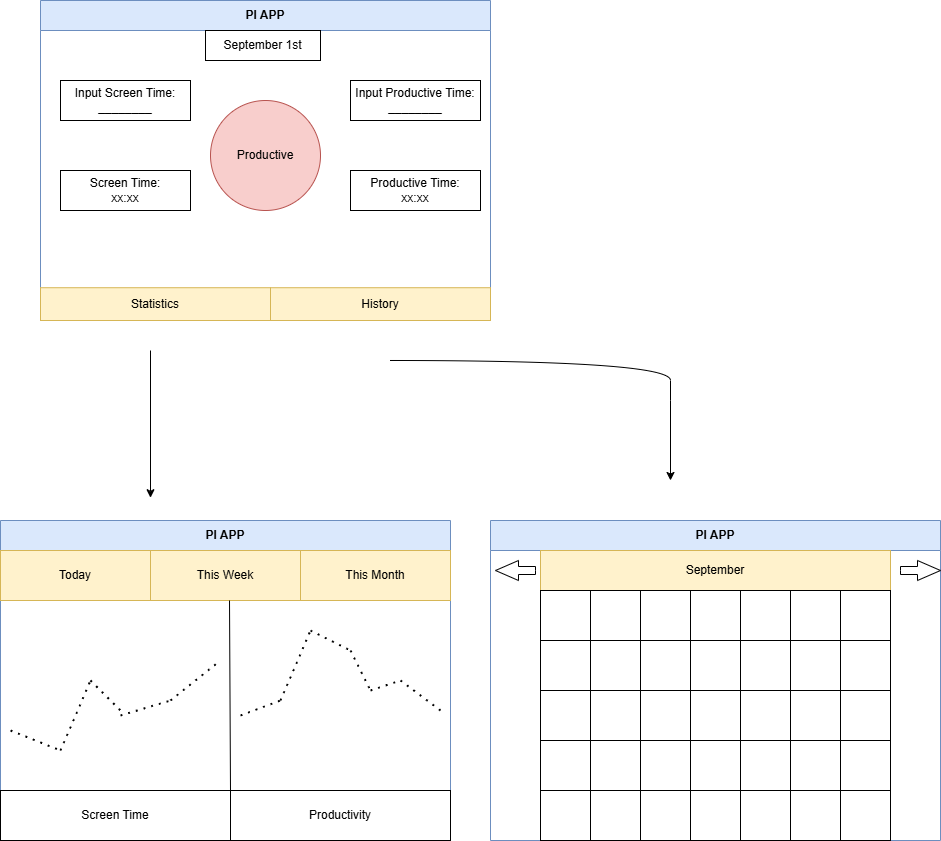
\includegraphics[width=0.75\linewidth]{UI Sketch.png}
    \caption{First Diagram}
    \label{fig:enter-label}
\end{figure}

\newpage
The first diagram showcased a tabular GUI with all the basic functionality that we had considered at the time.  


\section{Software Testing (Verification) (2 pages)}
Authors: James
\label{sec:testing}
\subsection{Test Plans}
These test plans will be used to test the completeness of the system, to ensure that it is robust and that nothing unexpected occurs. This includes checking the inputs of the user and ensuring that all outputs, such as graphs, are as expected, even in the case of data that may not be valid. These tests will be performed using the following types:

\begin{itemize}
    \item {Unit Testing}: Using pytest for components
    \item {Integration Testing}: Making sure that various services work well together (For example json files)
    \item {Functional Testing}: Manual validation
    \item {Performance Testing}: Using timers and looking at the performance of various sections
\end{itemize}

The first set of tests will be based on the validation of user inputs.
\begin{table}[h]
    \centering
    \renewcommand{\arraystretch}{1.3} % Adjust row spacing for readability
    \begin{tabular}{|l|l|p{9cm}|}
        \hline
        \textbf{ID} & \textbf{Test Case} & \textbf{Description} \\
        \hline
        1.1 & Manual data NaN errors  & Inputting characters that are not able to be parsed as numbers must prompt the user to re-enter data.\\
        \hline
        1.2 & Timers and overflow & If the timer overflows beyond 24 hours (for example in the case of the user forgetting to turn off the timer), this should be recognised and fixed appropriately.\\
        \hline
        1.3 & Negative goal input & Reject goals that are not feasible and prompt the user to re-enter data.\\
        \hline
        1.4 & Data durability & Ensure that data entered stays even after the application restarts.\\
        \hline
        1.5 & Stress test & Simulate 1000 timer starts/stops to make sure that memory does not leak.\\
        \hline
        1.6 & Inputting dates & When inputting a date that has not been logged or has not occurred yet, it should prompt the user to re-enter.\\
        \hline
        1.7 & Loading data & It is able to load data into the program from the JSON file without resulting in loss of data.\\
        \hline
    \end{tabular}
    \caption{validation of input}
    \label{tab:input_tests}
\end{table}
\\
\\
The next set of tests will be based on outputs to screen and the calculations that are needed to do so.
\\
\\

\begin{table}[h]
    \centering
    \renewcommand{\arraystretch}{1.3} % Adjust row spacing for readability
    \begin{tabular}{|l|p{10cm}|}
        \hline
        \textbf{Test No. Test} & \textbf{Description} \\
        \hline
        2.1 Screen/productive display & Ensure that the UI shows the same values as stored.\\
        \hline
        2.2 Productivity & Validate calculation by hand using raw data when calculating the increase in productivity.\\
        \hline
        2.3 null graphing & Ensure that the graph is able to render when there is no data.\\
        \hline
        2.4 graphs & Make sure that week ranges are able to select the correct ranges.\\
        \hline
        2.5 Graph performance & It takes less than a second for a graph to be rendered onto the screen\\
        \hline
    \end{tabular}
    \caption{validation of output}
    \label{tab:output_tests}
\end{table}

\newpage
\section{Reflection and Conclusion (4 pages)}
Authors:
\label{sec:reflection}
\subsection{System Critique}

\subsection{Process Critique}


%=== REFERENCES (does not count towards page limit) ===
\newpage
\section*{References}
Nasrullah, S. and Khan, M.S., 2015. The impact of time management on the students’ academic achievements. Journal of Literature, Languages and Linguistics, 11, pp.66–71. Available at: \url{https://core.ac.uk/reader/234693030} [Accessed 24 March 2025]
\\
\\
Betwick B, Koutsopoulou G, Miles J, Slaa E, Barkham M., 2010. Changes in undergraduate students' psychological well-being as they progress through university. Studies in Higher Education, 35(6), pp.633. Available at: \url{https://doi.org/10.1080/03075070903216643} [Accessed 24 March 2025].
\\
\\
Kersten-van Dijk, E.T., Westerink, J.H.D.M., Beute, F., and IJsselsteijn, W.A., 2016. Personal Informatics, Self-Insight, and Behavior Change: A Critical Review of Current Literature. Behaviour \& Information Technology, 35(7), pp. 268. Available at: \url{https://doi.org/10.1080/07370024.2016.1276456}  
[Accessed 24 March 2025].
\\
\\
Li, I., Dey, A. and Forlizzi, J., 2010. A Stage-Based Model of Personal Informatics Systems. ACM Transactions on Computer-Human Interaction, pp. 557-565. Available at: \url{https://doi.org/10.1145/1753326.1753409} [Accessed 24 March 2025]
\\
\\
Epstein, D.A., Caraway, M., Johnston, C., Ping, A., Fogarty, J., and Munson, S.A., 2016. Beyond Abandonment to Next Steps: Understanding and Designing for Life after Personal Informatics Tool Use, pp.1112. Available at: \url{https://doi.org/10.1145/2858036.2858045} 
[Accessed 24 March 2025]
\\
\\
Rapp, A., Marcengo, A., Buriano, L., Ruffo, G., Lai, M., and Cena, F., 2018. Designing a personal informatics system for users without experience in self-tracking: a case study. Behaviour \& Information Technology, pp.337. Available at: \url{https://doi.org/10.1080/0144929X.2018.1436592} 
[Accessed 24 March 2025].


%=== APPENDICES ===
\newpage
\appendix

\section{Sprints}

\subsection{Sprint 1}
\subsubsection{Report & Planning}

\renewcommand{\arraystretch}{1.3}
\begin{tabular}{|c|p{12cm}|}
\hline
\textbf{Task} & \textbf{Description} \\
\hline
A1 & Complete Introduction of the report: Background Research of the problem, and introduce our PI system \\
\hline
A2 & Partially complete Agile software section, focus on planning the sprint section \\
\hline
A3 & Start Software Requirements Specification: Use the introduction as well primary research through google forms to ask the users on what type of functional requirements they need \\
\hline
A4 & Design Section: Start planning out UML diagrams on how the code should look like \\
\hline
A5 & Software testing: Create Test plans \\
\hline
A6 & Maintain updated reference list \\
\hline
A7 & Include screenshots of tables in appendix \\
\hline
\end{tabular}

\subsubsection{Development & Coding}

\subsection{Sprint 2}
\subsubsection{Report & Planning}
\renewcommand{\arraystretch}{1.3}
\begin{tabular}{|c|p{12cm}|}
\hline
\textbf{Task} & \textbf{Description} \\
\hline
C1 & Finish Agile Software Process Planning and Management section \\
\hline
C2 & Update design section with screenshots of final UI \\
\hline
C3 & Complete testing for Sprint 2 \\
\hline
C4 & Write project conclusion and future improvements \\
\hline
C5 & Collect final user feedback for evaluation \\
\hline
C6 & Finalise and format the complete report for submission \\
\hline
\end{tabular}
\subsubsection{Development & Coding}

\section{Group Contribution Form}
% Insert completed GCF

\section{Meeting Minutes}
% Attach meeting minutes

\section{Interview Transcripts}
% Include transcripts

\end{document}
